% !TeX root = ./../memoria.tex
\chapter{Diseño e implementación}

\label{Capitulo3}

En este capítulo se exponen las decisiones de diseño tomadas para la elaboración del robot propuesto. Se detallan las dimensiones de las piezas que constituyen el chasis, su esquema de conexiones eléctricas y finalmente la implementación del software y el firmware embebido.

\section{Estructura mecánica}

En esta sección se describe la estructura física del robot y se explican los criterios utilizados tanto para el dimensionamiento de piezas como para su disposición.

\subsection{Disposición en niveles}
Tal como se menciona en la sección \ref{sec:turtlebot}, el diseño propuesto toma como referencia a la base móvil \textit{open source} Turtlebot 2. Por este motivo, Lubobot también se compone de una base móvil cilindrica de tracción diferencial y la misma funciona como soporte para una estructura escalable en "niveles", gracias a a lo cual el usuario puede agregar nuevos componentes sin dificultad, según los requisitos particulares de su aplicación. En la figura \ref{fig:lubobotURDF} se muestra una representación en 3D de su estructura física en la configuración propuesta.

\begin{figure}[ht]
    \centering
    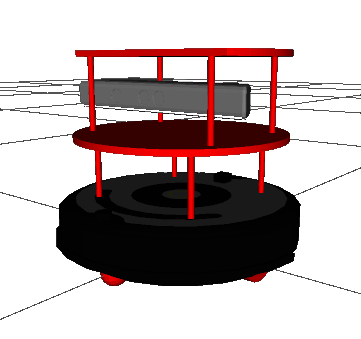
\includegraphics[scale=0.5]{./Figures/lubobot_urdf.png}
    \caption{Vista frontal del modelo URDF de Lubobot representado en RViz.}
    \label{fig:lubobotURDF}
\end{figure}

\newpage

Sobre la base móvil se montaron cuatro varillas roscadas de 5 mm de diámetro y 80 mm de largo, de las cuales las dos frontales fueron fijadas a la agarradera o  \textit{handler} del Roomba, mientras que las dos traseras se fijaron directamente al chasis. Dicha disposición fué calculada en base a las áreas del robot que el autor determinó como seguras para su modificación, es decir, que no representan un riesgo al buen funcionamiento de la base móvil.

\subsection{Disposición de componentes}

Los diferentes componentes funcionales del robot fueron dispuestos en la configuración que se aprecia en la figura \ref{fig:lubobotComponentes}, a excepción de la \textit{laptop}, presente para fines de ejemplo ya que representa un elemento opcional. Para esta disposición se tuvieron en cuenta los siguientes objetivos:

\begin{itemize}
  \item Mantener bajo el centro de gravedad del conjunto.
  \item Maximizar el espacio libre en el nivel superior para futuros \textit{upgrades}.
  \item Posicionar la IMU lo mas cerca posible del centro de rotación de la base.
  \item Posicionar el sensor Kinect a alrededor de 30 cm del suelo.
  \item Mantener sin obstrucciones el acceso al botón central del Roomba.
\end{itemize}

\begin{figure}[ht]
    \centering
    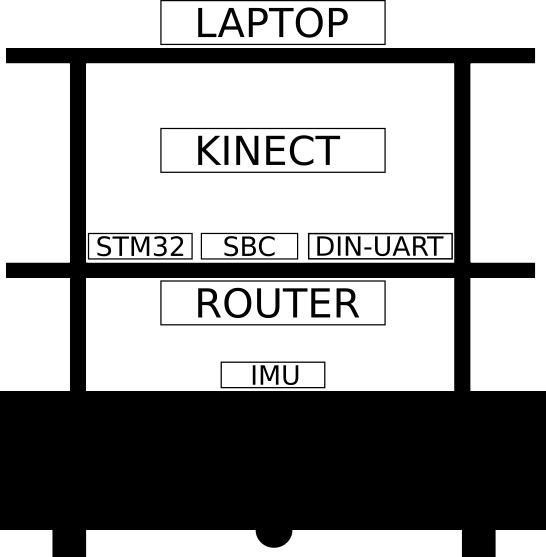
\includegraphics[scale=0.4]{./Figures/distribucion_componentes.png}
    \caption{Distribución de componentes del robot.}
    \label{fig:lubobotComponentes}
\end{figure}

\section{Diagrama en bloques de conexiones}

En la figura \ref{fig:lubobotComponentes} se muestra el diagrama de conexiones entre los distintos componentes electronicos que componen el sistema y se indica además, el protocolo utilizado para cada una de las mismas. Se decidió dotar al robot de un \textit{router} wifi a bordo de modo a facilitar su conexión con la computadora destinada a hacer de estación de control para el envío de misiones.

\begin{figure}[ht]
    \centering
    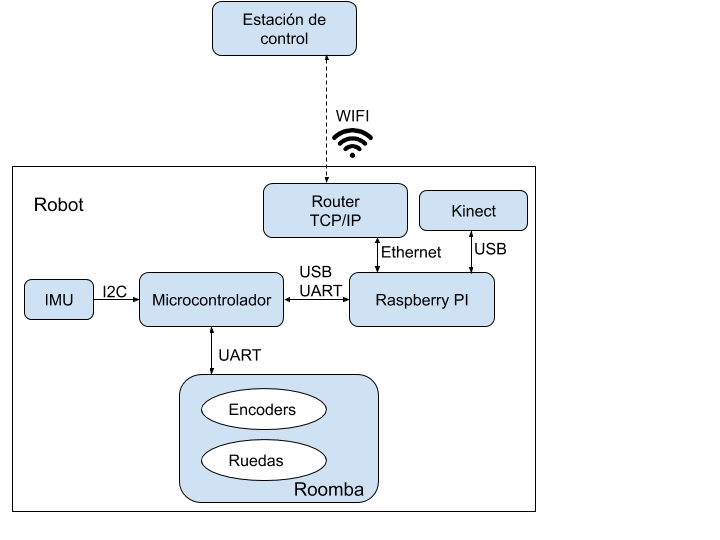
\includegraphics[scale=0.5]{./Figures/lubobot_conexiones.png}
    \caption{Diagrama de conexiones de los componentes constitutivos del robot.}
    \label{fig:lubobotComponentes}
\end{figure}

\newpage

\section{Implementación de firmware}

En esta sección se detallan las decisiones de diseño e implementación del firmware, encargado de la interconexión del robot Roomba y la Raspberry PI así como también de la lectura de sensores ajenos a la base móvil original como lo es la IMU.

\subsection{Distribución de tareas en FreeRTOS}

Debido a la necesidad de atender rutinas naturaleza tanto síncrona como asíncrona en el firmware, se decidió utilizar un RTOS para su implementación. Las tareas involucradas se describen a continuación, agrupadas en base a su responsabilidad dentro del sistema.

\subsection{Interfaz Roomba-microcontrolador}

Este conjunto de tareas cumplen la función de \textit{proxy} entre la base móvil Roomba y el resto del sistema. El microcontrolador se ocupa de la serialición y des-serialización de los paquetes intercambiados con el robot mediante el protocolo Open Interface, detallado en la sección \ref{sec:openInterface}. Las tareas responsables del manejo de esta función se describen en el apartado siguiente.

\begin{itemize}
  \item \textbf{Solicitud de lectura de sensores}: realiza la lectura de cada uno de los dos encoders disponibles de manera periódica cada 100 ms, actualizando las variables internas de estado en cada iteración con el valor actualizado.
  \item \textbf{Envío de comandos a actuadores}: realiza el despacho de comandos a los distintos actuadores disponibles en base a las órdenes recibidas desde ROS. Si bien esta tarea puede considerarse de carácter asíncrono, se implementó en la misma un mecanismo de \textit{watchdog} para evitar que un posible fallo en la comunicación con ROS ponga en peligro la integridad del usuario y del robot. Para esto, la tarea verifica cada 100 ms la existencia de un comando de velocidad nuevo. En su ausencia, envía una orden para detener el robot.
\end{itemize}

\subsection{Interfaz microcontrolador-ROS}

Esta interfaz involucró la migración de la librería rosserial, mencionada en la sección \ref{sec:rosserial}, la cual posibilita entablar una comunicación serial asíncrona entre el microcontrolador y ROS utilizando el protocolo de mensajes estandar del \textit{framework}.


\section{Implementación de software}

\subsection{Paquete Lubobot para ROS}

\subsection{IMU y estimador de orientación}

\subsection{Odometría basada en encoders}

\subsection{Matriz de covarianza}

\subsection{Configuración del paquete ros\_localization}

\subsection{Configuración del paquete de navegación de ROS}
 
